\begin{figure}[h]
    \centering
    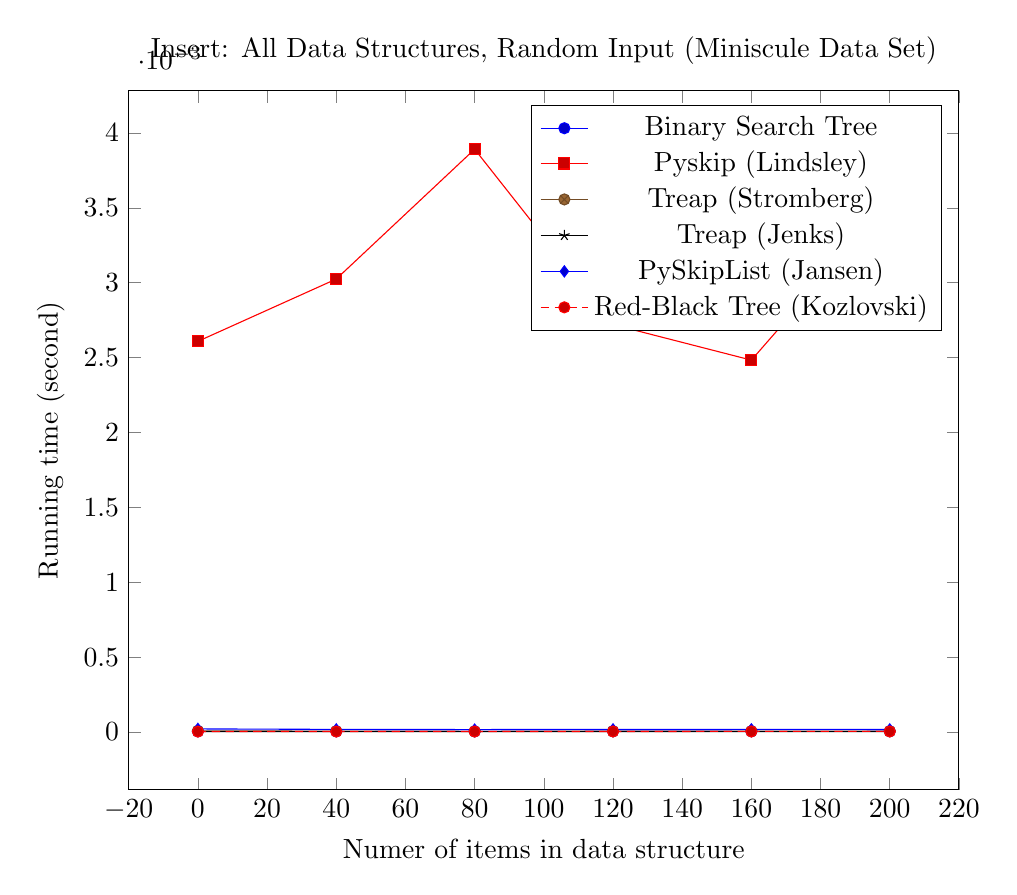
\begin{tikzpicture}
        \begin{axis}[
            xlabel={Numer of items in data structure},
            ylabel={Running time (second)},
            title={Insert: All Data Structures, Random Input (Miniscule Data Set)},
            width=\textwidth
        ]
		\addplot coordinates {
			(0, 3.885161844097151e-06)
			(40, 4.005631978787338e-06)
			(80, 3.824926776752058e-06)
			(120, 4.57786511862679e-06)
			(160, 4.397159916580406e-06)
			(200, 4.427277450247402e-06)
		};
		\addplot coordinates {
			(0, 0.0026083290039378704)
			(40, 0.003024432849193981)
			(80, 0.0038913660560336736)
			(120, 0.0027200048188053883)
			(160, 0.002482889476180805)
			(200, 0.003541821960199676)
		};
		\addplot coordinates {
			(0, 7.710088620838108e-06)
			(40, 5.330803460501521e-06)
			(80, 4.306807315557215e-06)
			(120, 4.9091579890525596e-06)
			(160, 5.2103333258113335e-06)
			(200, 5.2705683931453254e-06)
		};
		\addplot coordinates {
			(0, 2.680460497073156e-06)
			(40, 2.469637761381982e-06)
			(80, 2.2286974919571987e-06)
			(120, 2.319050093002595e-06)
			(160, 2.1082273572448074e-06)
			(200, 2.6202254297391647e-06)
		};
		\addplot coordinates {
			(0, 2.035945276439577e-05)
			(40, 1.716699419485046e-05)
			(80, 1.5932175314148367e-05)
			(120, 1.737781693056384e-05)
			(160, 1.767899226732261e-05)
			(200, 1.7106759127494266e-05)
		};
		\addplot coordinates {
			(0, 2.6804604970953604e-06)
			(40, 2.9515183001649346e-06)
			(80, 3.0719884348773264e-06)
			(120, 3.433398838970092e-06)
			(160, 3.4936339063040834e-06)
			(200, 3.493633906326288e-06)
		};
        \legend{Binary Search Tree, Pyskip (Lindsley), Treap (Stromberg), Treap (Jenks), PySkipList (Jansen), Red-Black Tree (Kozlovski)}
        \end{axis}
    \end{tikzpicture}
    \caption{Average of 10 operations, benchmarked every 40, starting at 0.}
\end{figure}